\documentclass{article} % Definisi jenis dokumen

%%%%% Definisi paket-paket yang seharusnya digunakan %%%%%
\usepackage[utf8]{inputenc} % paket encoding input utf8
\usepackage[T1]{fontenc} % paket encoding huruf latin

%%%%% Definisi paket-paket yang digunakan sesuai kebutuhan %%%%%
\usepackage[yyyymmdd,hhmmss]{datetime} % paket tanggal-waktu
\usepackage{graphicx} % paket grafik/gambar
\usepackage[english]{babel} % paket modifikasi label/caption pada bahasa tertentu
\usepackage{geometry} % paket ukuran kertas dan margin
\usepackage{tabularray}
\usepackage{hyperref}
\usepackage{float}
\usepackage{caption}

%%%%% Pengaturan ukuran kertas dan margin %%%%%
\geometry{
	a4paper,
	left=10mm,
	right=10mm,
	top=15mm,
	bottom=15mm,
}

%%%%% Pengaturan perintah informasi perangkat lunak (hanya untuk GNU/Linux) %%%%%
\newcommand{\ShowOsVersion}{
	\immediate\write18{\unexpanded{foo=`uname -sro` && echo "${foo}" > tmp.tex}}
	\input{tmp}\immediate\write18{rm tmp.tex}
}

\newcommand{\ShowTexVersion}{
	\immediate\write18{\unexpanded{foo=`pdflatex -version | head -n1 | cut -d' ' -f1,2` && echo "${foo}" > tmp.tex}}
	\input{tmp}\immediate\write18{rm tmp.tex}
}

\begin{document}
%%%%%%%%%%%%%%%%%%%%%%%%%%%%%%%%%%%%%%%%%%%%%%%%%%%%%%%%%%%%%%%%%

	\begin{titlepage}

		\centering % untuk membuat tengah teks

		{
			\LARGE % pakai font besar
			\bf % pakai font BOLD
			Rekapitulasi Nota Kegiatan
		}

		\bigskip
		{\Large \bf Achmadi ST MT}
		\vfill % menambahkan ruang kosong vertikal

		\raggedright
		\noindent Buku ini ditulis dengan:\\ % tanda \\ menambahkan garis baru
		OS : \ShowOsVersion \\
		TeX : \ShowTexVersion \\
		Update: {\today} at \currenttime\\
	\end{titlepage}

	%%%%%%%%%%%%%%%%%%%%%%%%%%%%%%%%%%%%%%%%%%%%%%%%%%%%%%%%%%%%%%%%%

	\section{Tabel Rekapitulasi}
	
	\subsection{Transportasi}
	
	\begin{table}[H]
		\centering
		\begin{tabular}{|c|c|c|c|c|c|}
			\hline
			Items & Qty & Total & Shop & Paid & URL \\
			\hline
			Bus Kota & 6 & Rp. 30.000 & Bus-Suroboyo & Mas Deni & \hyperlink{https://tiketresmi.com/suroboyo-bus/}{Info-Traif} \\
			Bus Antar-Kota & 6 & Rp. 360.000 & Restu & 4/6 Mas Deni & - \\
			Penginapan & 1 & Rp. 150.000 & Red-Doorz & Mas Deni & - \\
			Penginapan & 1 & Rp. 198.000 & Red-Doorz & Mas Deni & - \\
			\hline
			\textbf{Total} & & Rp. 738.000 & - & - & - \\
			\hline
		\end{tabular}
	\end{table}

	\subsection{Prototype}

	\begin{table}[H]
	\centering
	\begin{tabular}{|c|c|c|c|c|c|}
		\hline
		Items & Qty & Total & Shop & Paid & URL \\
		\hline
		Opto-Encoder & 3 & Rp. 24.000 & Akhi-Shop Surabaya &  - & \hyperlink{https://www.tokopedia.com/akhishop/opto-coupler-encoder-sensor-module}{Tokopedia} \\
		Box-Plastic & 3 & Rp. 24.600 & Eltech Surabaya & - & \hyperlink{https://www.tokopedia.com/eltech-online/box-electronic-instrument-project-plastic-03-15-cream-40x84x142mm}{Tokopedia} \\
		Diode-Regulator & 12 & Rp. 5.100 & Mulsanne Surabaya & - & \hyperlink{https://www.tokopedia.com/mulsanne/ic-ams1117-5-volt-step-down-smd-800ma}{Tokopedia} \\
		Sabut Kawat & 1 & Rp. 7.200 & Alfamart Madiun & - & - \\
		Tang-Kabel, Komponen & - & Rp. 52.000 & Bintang-Mas Madiun & Mas Deni & - \\
		Komponen & - & Rp. 21.000 & Bintang-Mas Madiun & Mas Deni & - \\
		Komponen & - & Rp. 15.000 & Berkat Surabaya & - & - \\
		Komponen & - & Rp. 16.000 & Berkat Surabaya & - & - \\
		Komponen & - & Rp. 100.900 & Digiware Surabaya & - & \hyperlink{https://digiwarestore.com/id/}{Digiware} \\
		FT232RL & 2 & Rp. 102.100 & Digiware Surabaya & - & \hyperlink{https://digiwarestore.com/id/serial-communication/ft232rl-166019.html}{Digiware} \\
		Cap 0.1uF & 20 & Rp. 10.000 & Digiware Surabaya & - & \hyperlink{https://digiwarestore.com/id/smd-capacitor/01uf-50v-10-0805-t-241110.html}{Digiware} \\
		Potong Akrilik & 6 & Rp. 30.000 & Embong-Malang Surabaya & - & - \\
		PCB Versi 1 & 3 & Rp. 298.800 & Raftech & - & \hyperlink{https://www.tokopedia.com/raftech/jasa-cetak-pcb-double-layer-fr4-full-masking-jalur-masking-silkscreen}{Tokopedia} \\
		PCB Versi 2 & 3 & Rp. 371.300 & Gerai-Cerdas & - & \hyperlink{https://www.tokopedia.com/geraicerdas/cetak-pcb-1-keping-single-double-layer-rapid-prototyping-satuan}{Tokopedia} \\
		STM32F103RB & 4 & Rp. 180.000 & Shenzhen China & - & \hyperlink{https://id.aliexpress.com/item/1005002651134172.html}{Aliexpress} \\
		\hline
		\textbf{Total} & & Rp. 1.204.000 & - & - & - \\
		\hline
	\end{tabular}
	\end{table}

	\subsection{Konsumsi}
	
	\begin{table}[H]
		\centering
		\begin{tabular}{|c|c|c|c|c|c|}
			\hline
			Items & Qty & Total & Shop & Paid & URL \\
			\hline
			Roti Gembul & 2 & Rp. 37.000 & Gembul Madiun & Mas Deni & - \\
			Telur & 10 & Rp. 24.000 & Alfamart & - & - \\
			Telur & 6 & Rp. 21.000 & Alfmart & - & - \\
			\hline
			\textbf{Total} & & Rp. 82.000 & - & - & - \\
			\hline
		\end{tabular}
	\end{table}

	\newpage
	\section{Scan Nota}

	\begin{figure}[H]
		\centering
		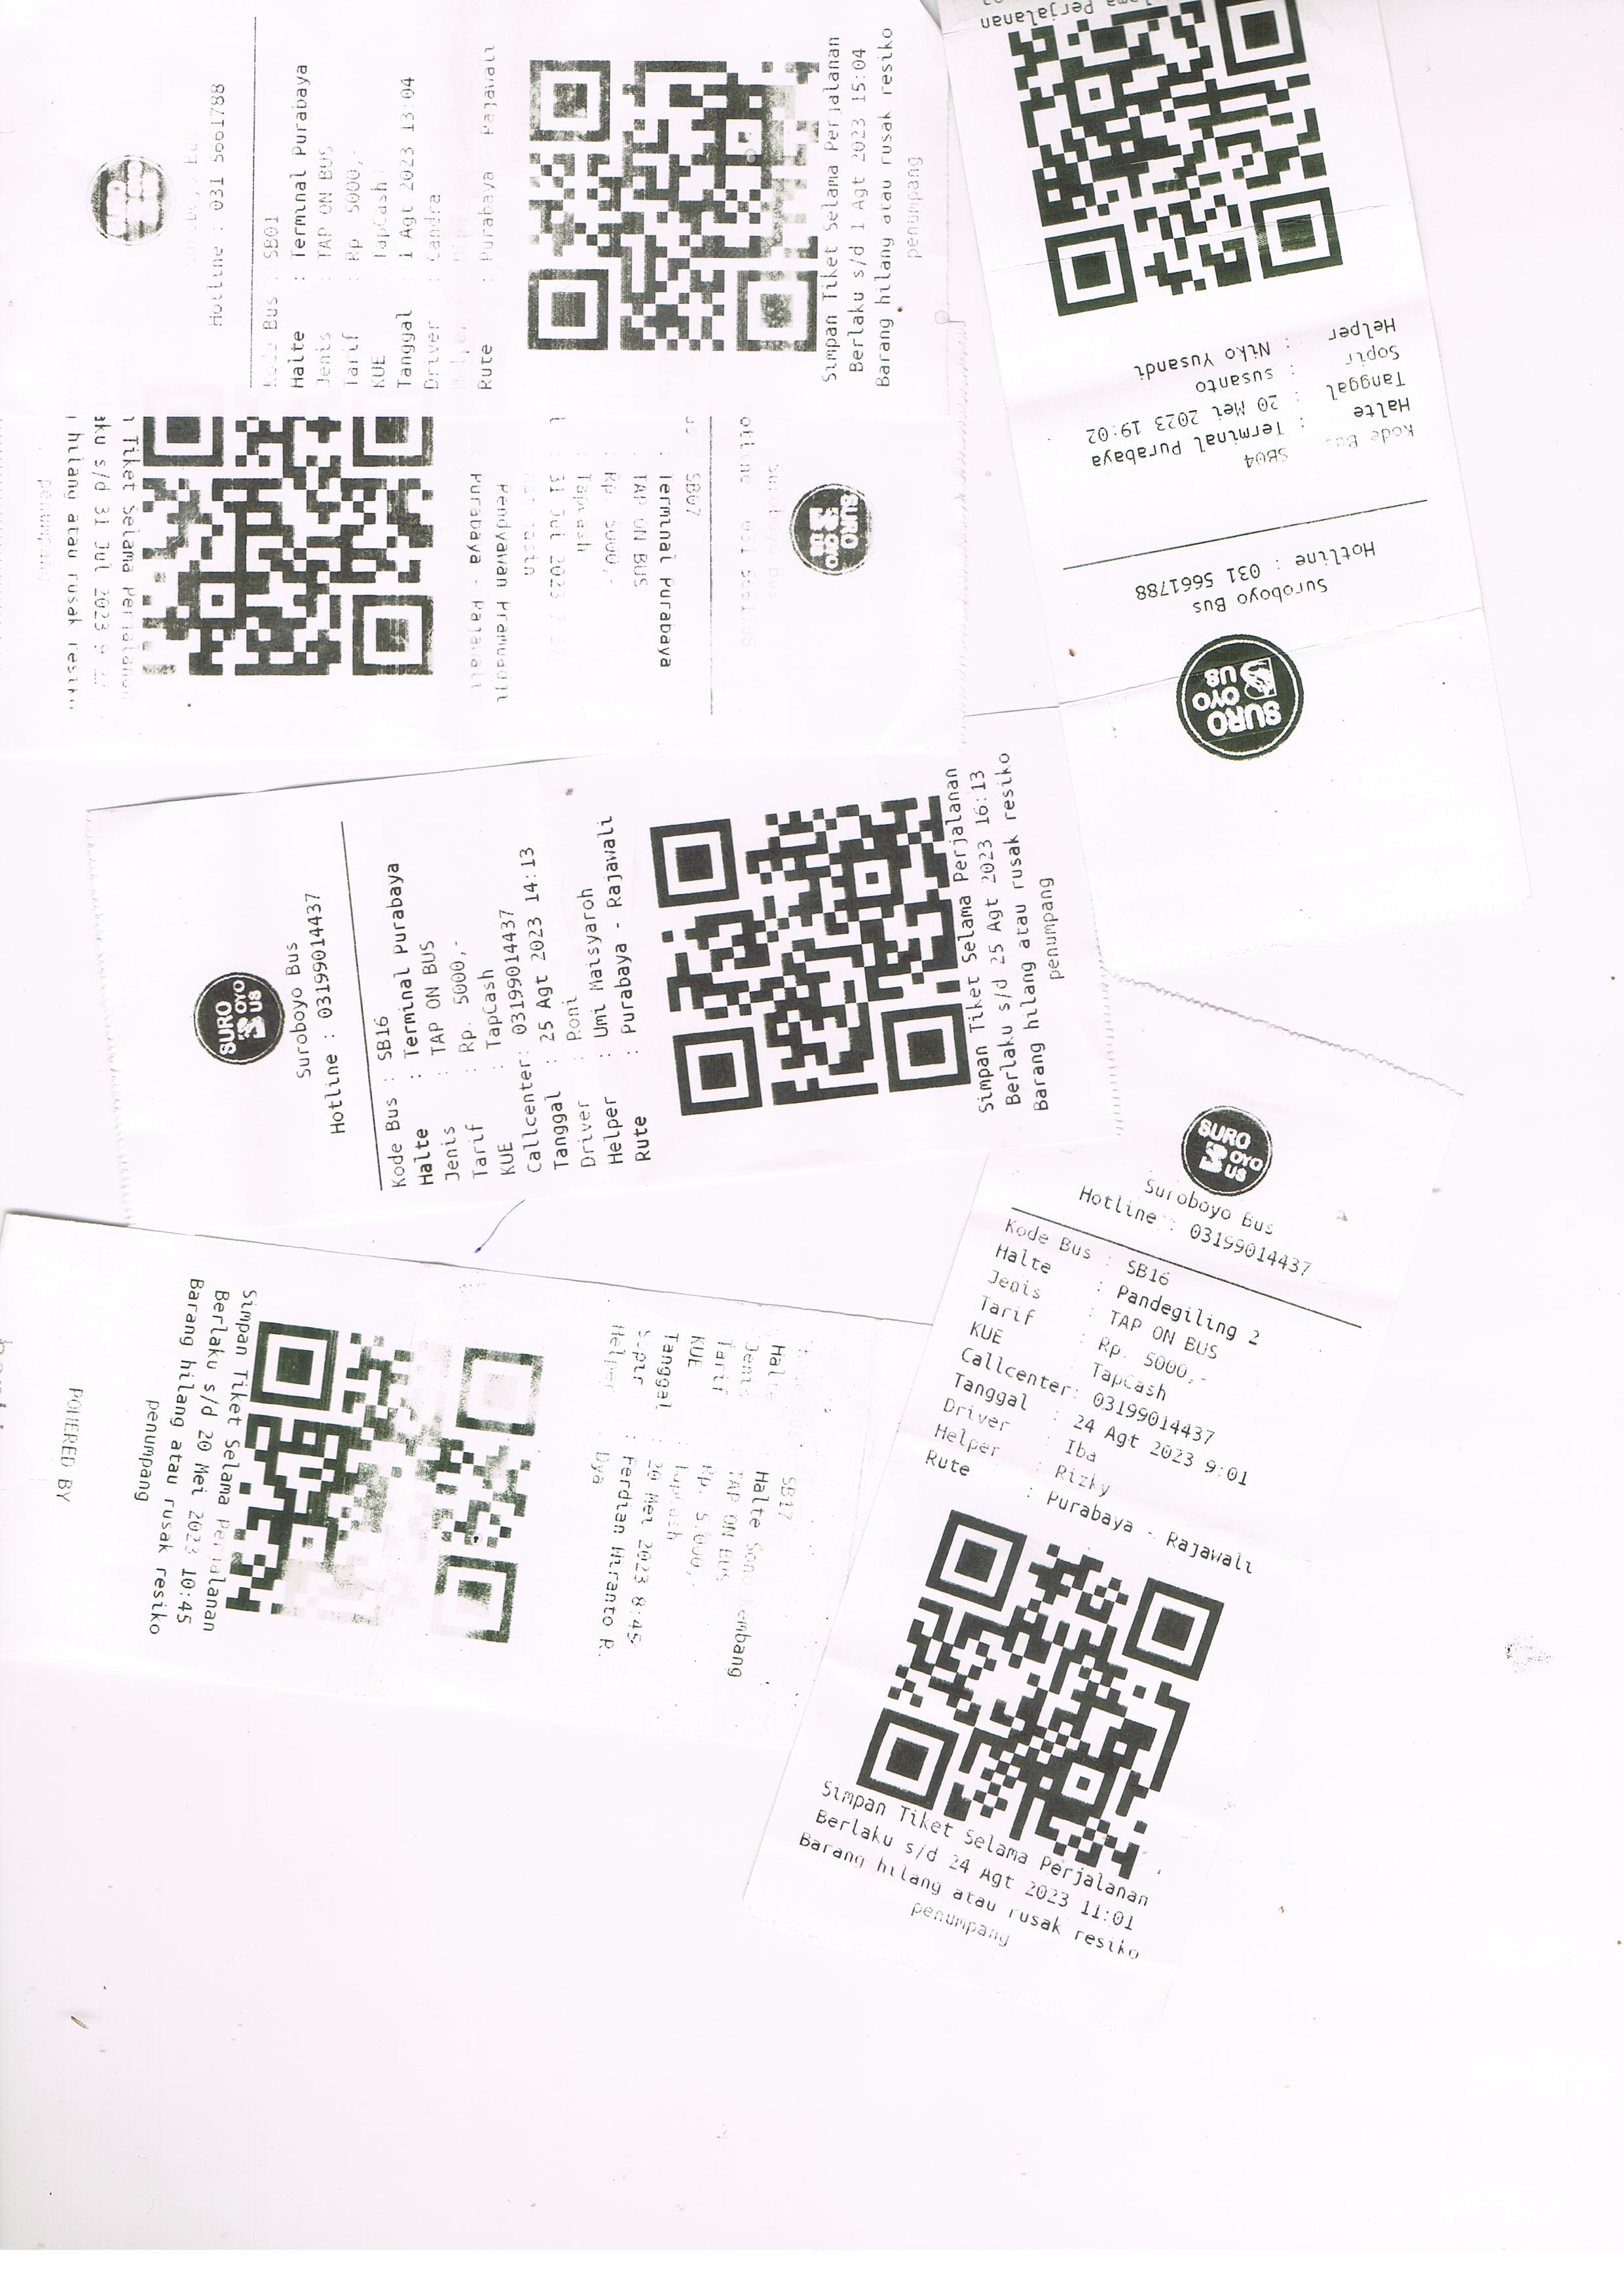
\includegraphics[width=0.8\textwidth]{images/bus_sby}
	\end{figure}

	\begin{figure}[H]
		\centering
		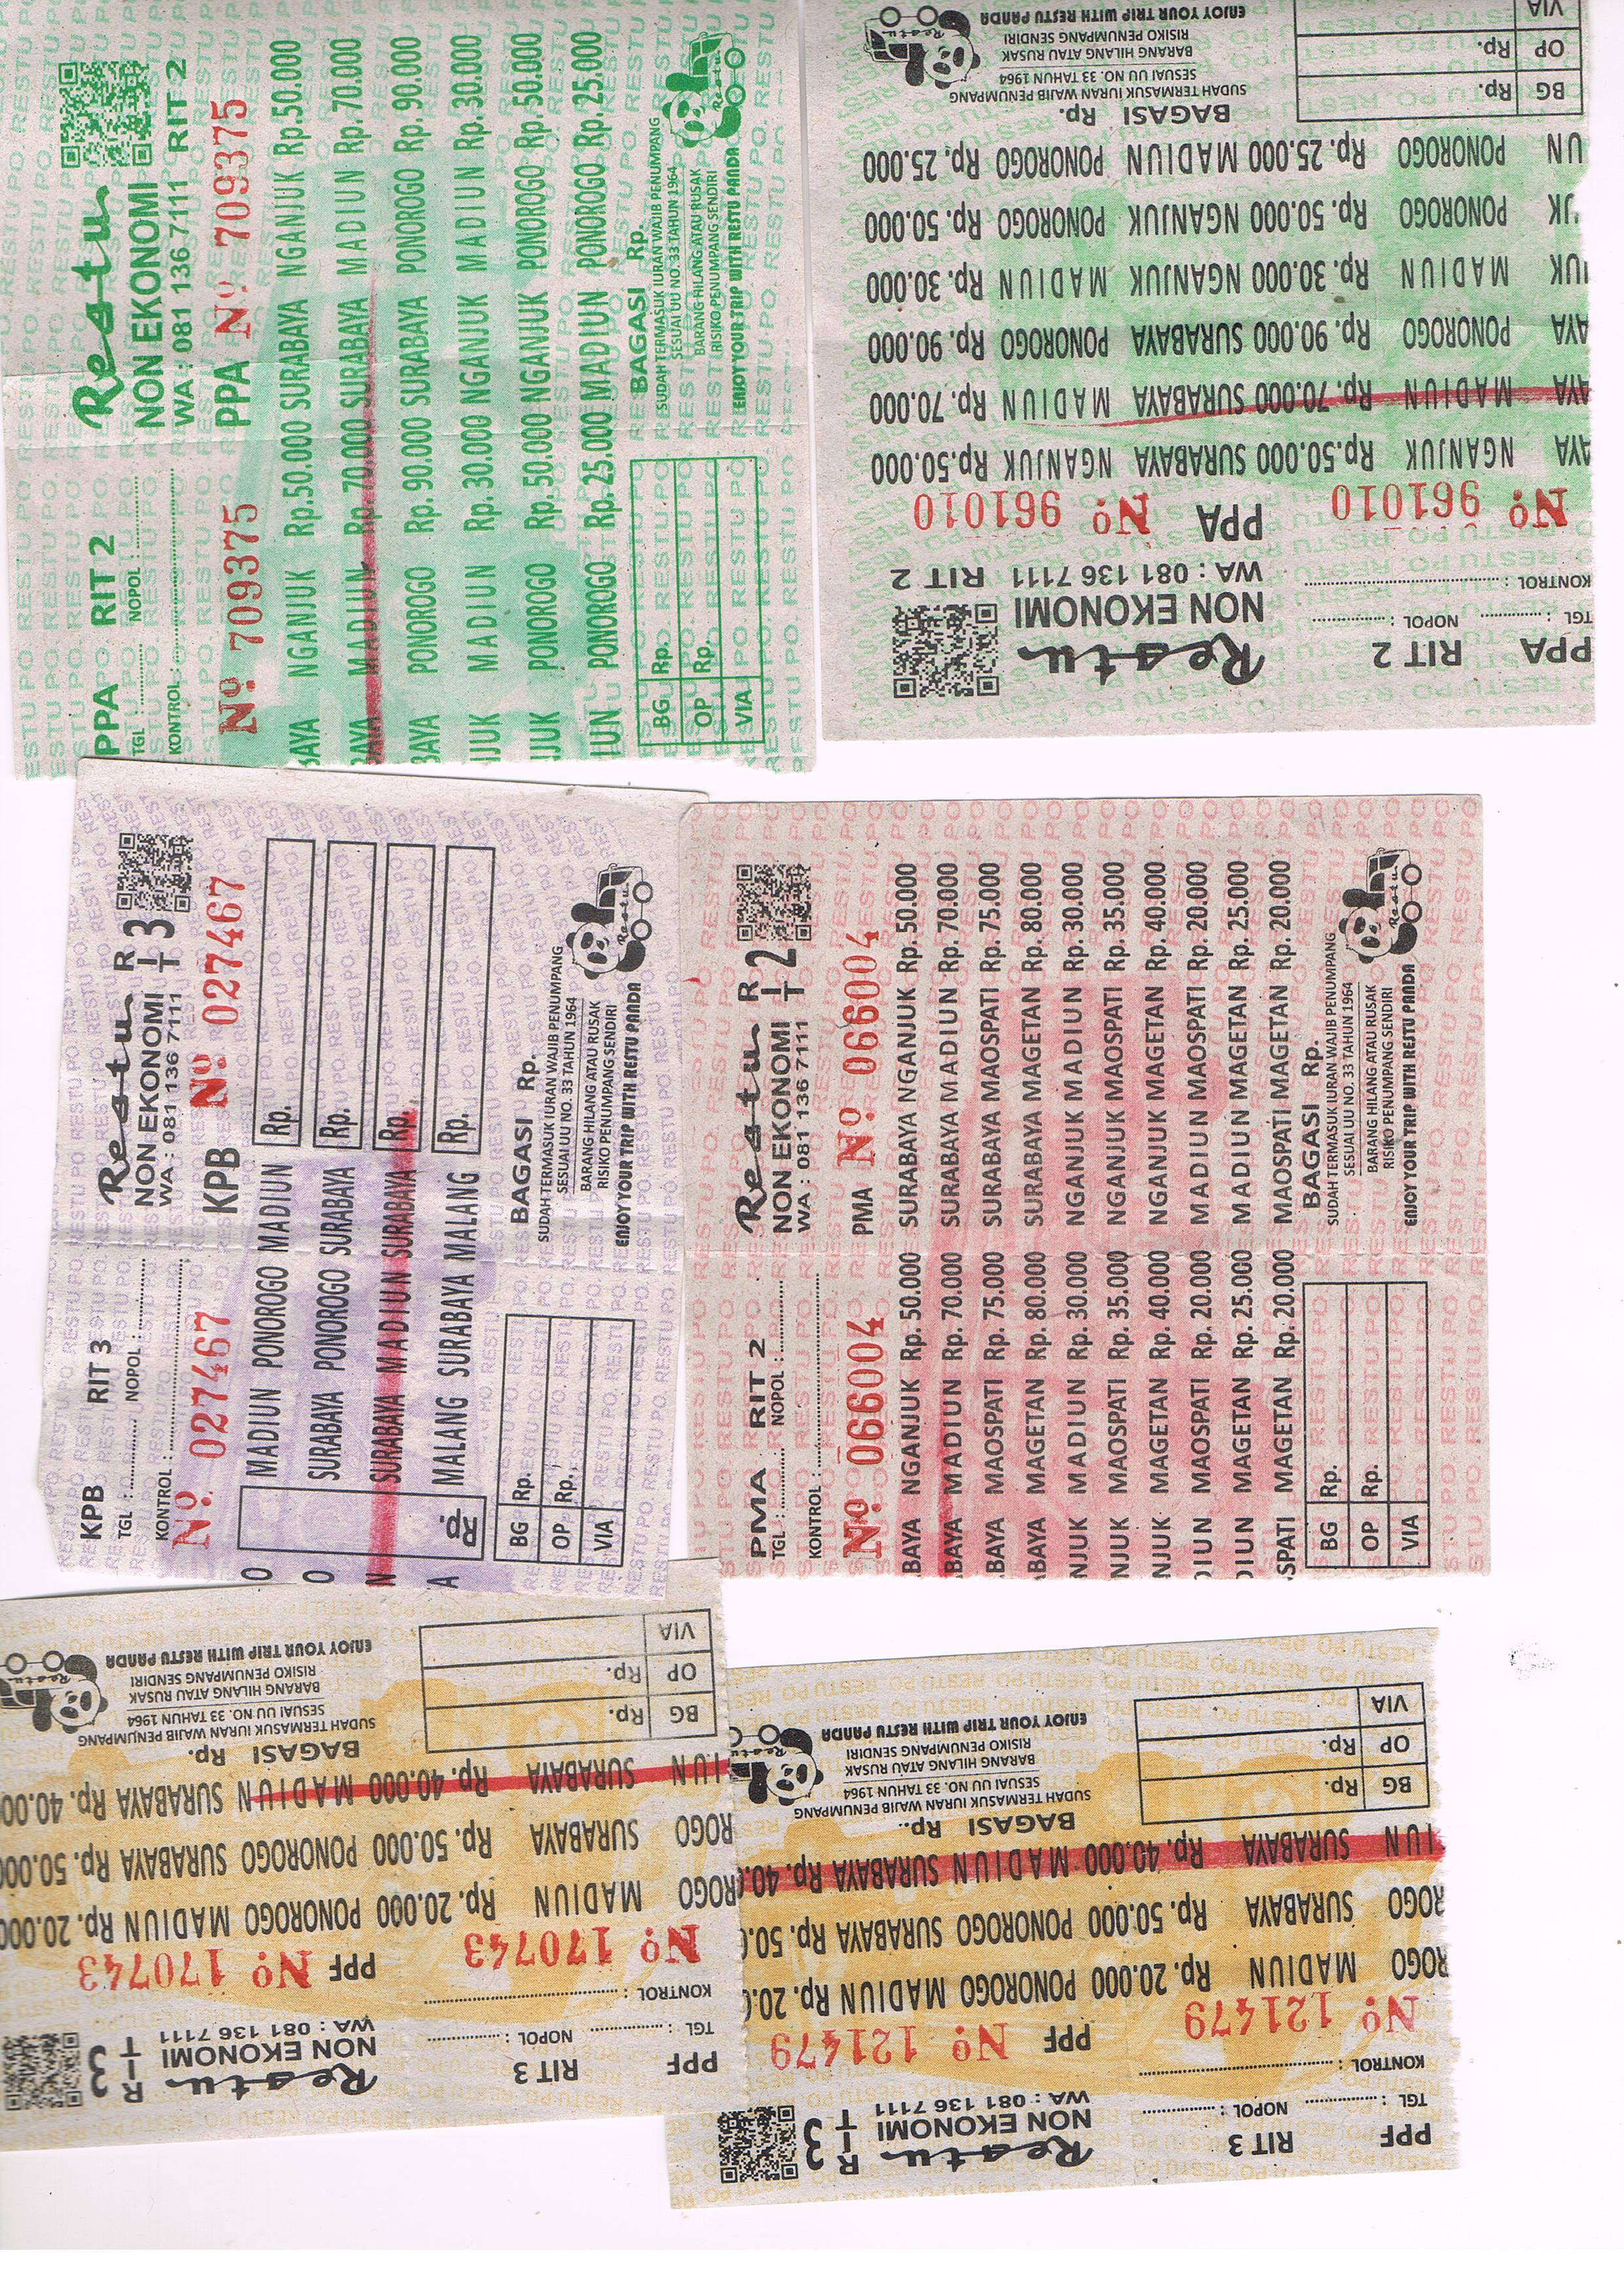
\includegraphics[width=0.8\textwidth]{images/bus_madiun}
	\end{figure}

	\begin{figure}[H]
		\centering
		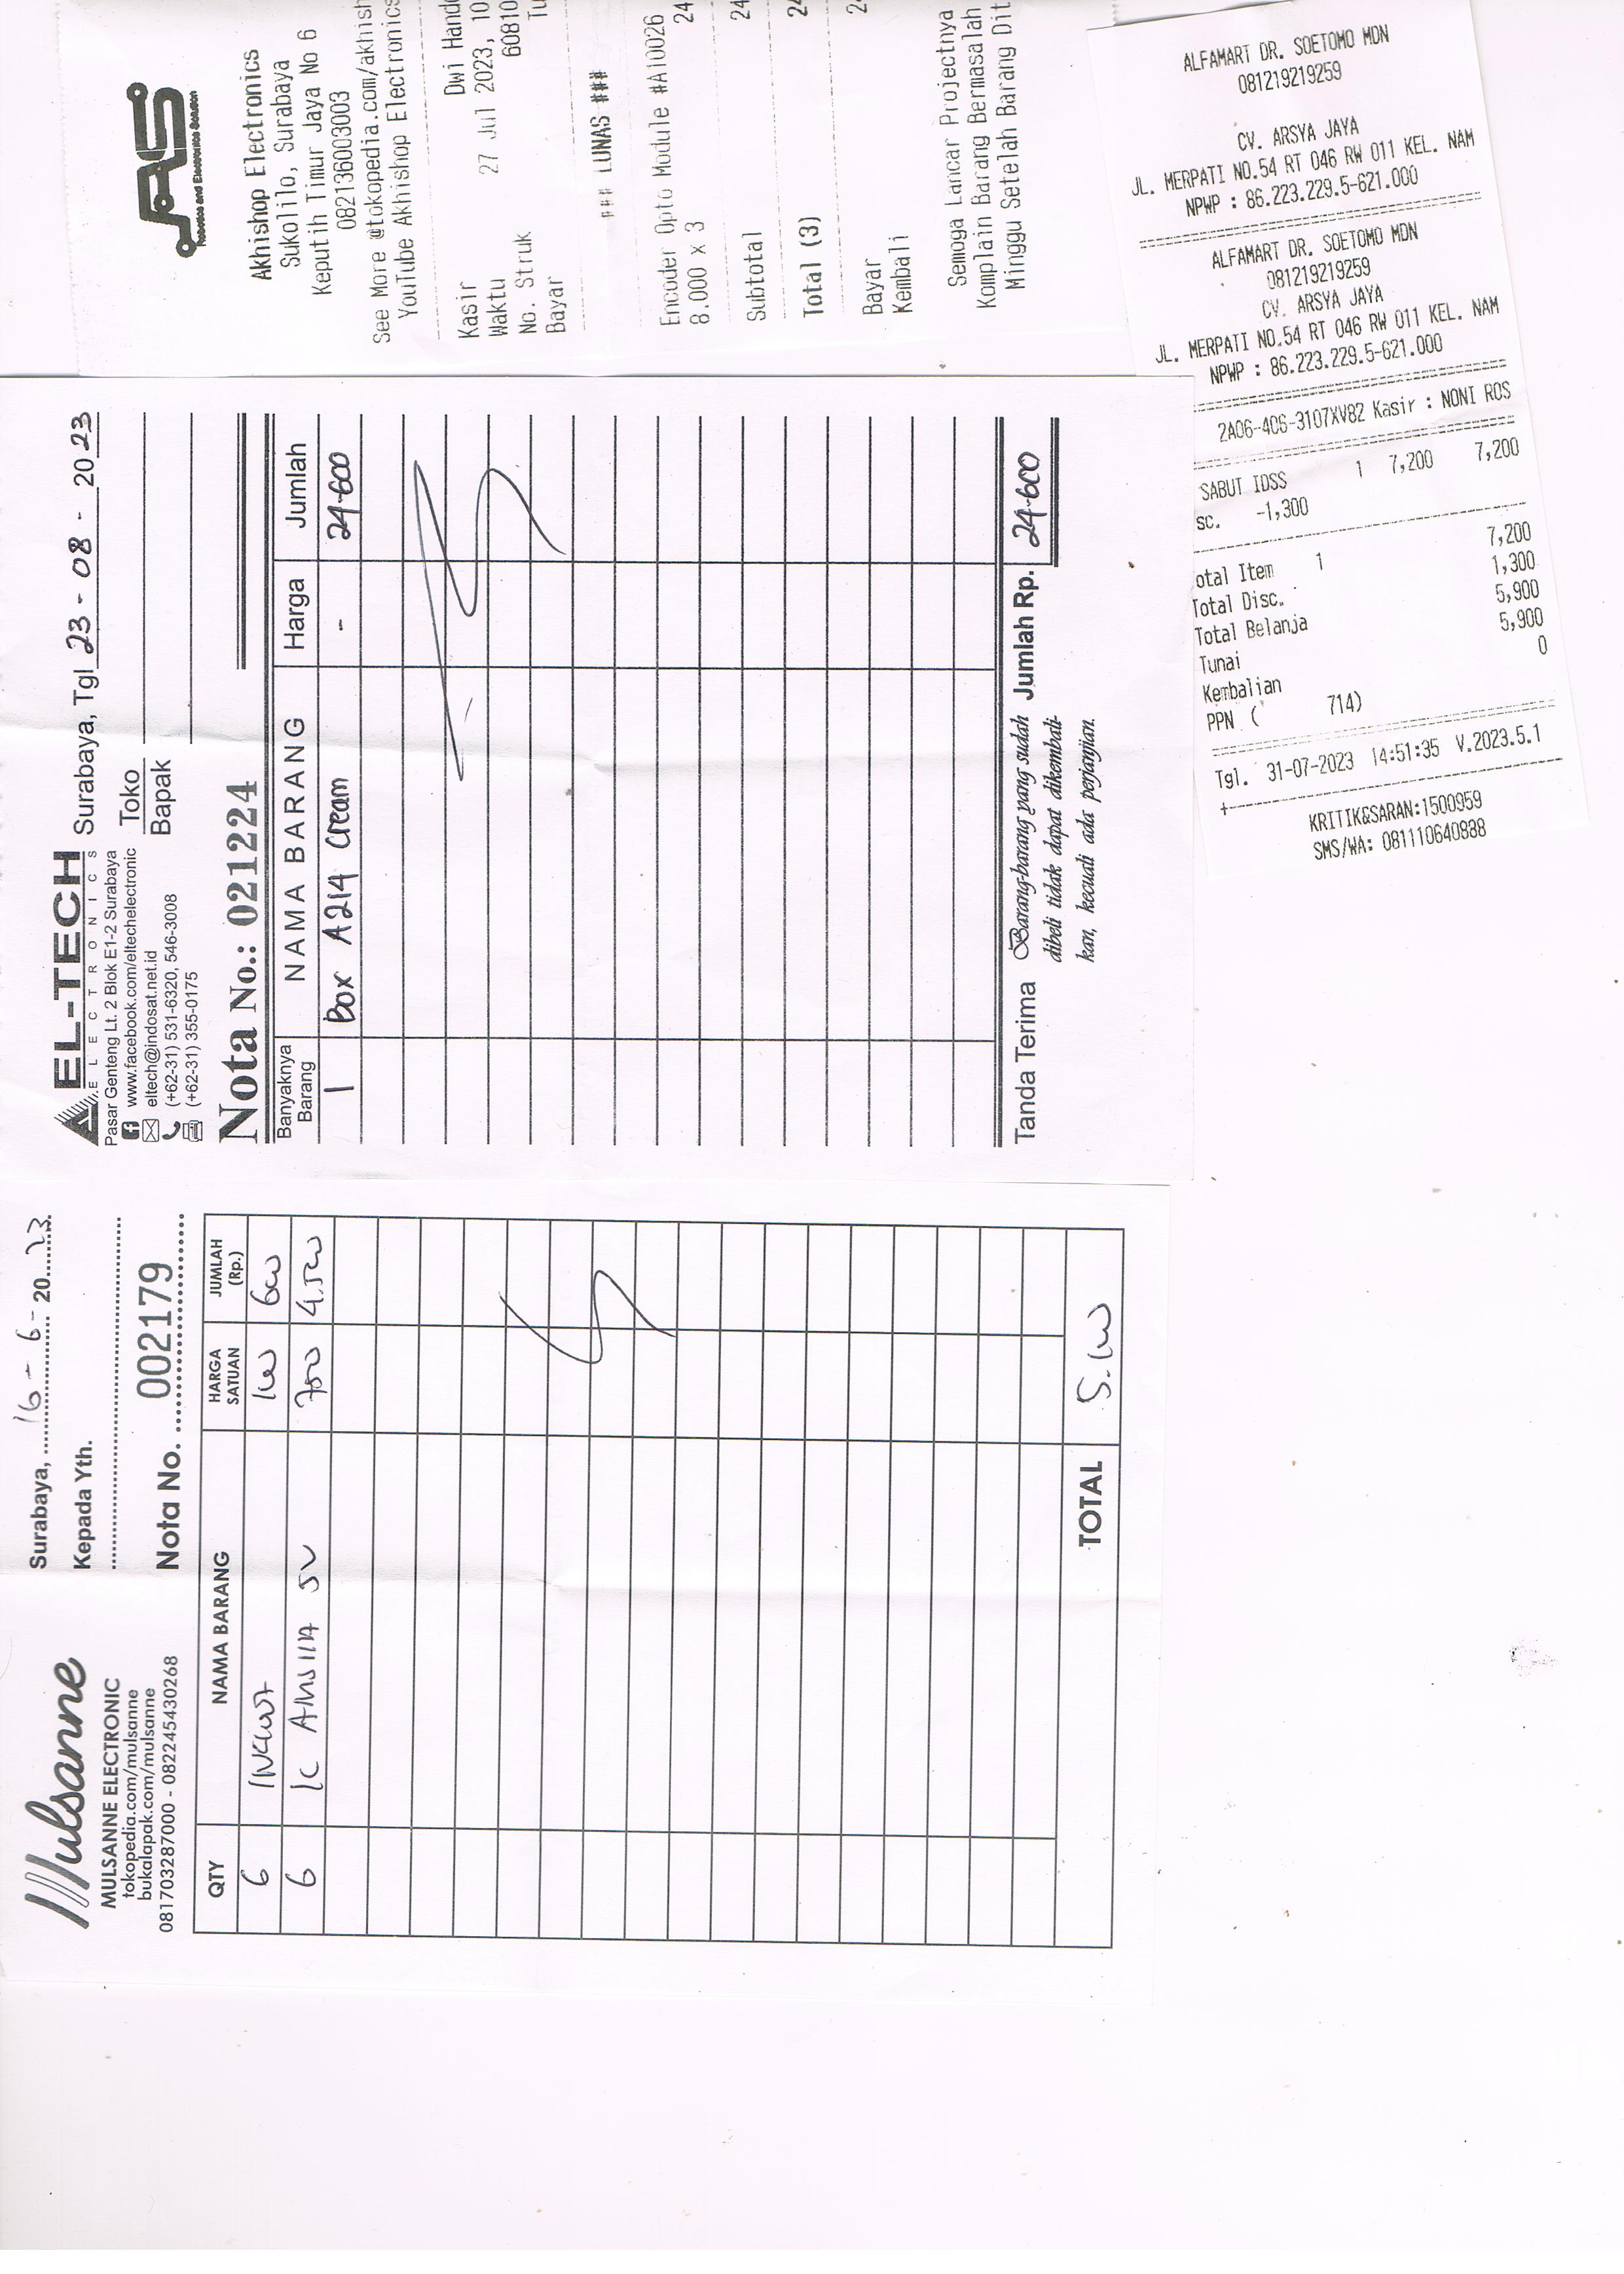
\includegraphics[width=0.8\textwidth]{images/komponen0}
	\end{figure}

	\begin{figure}[H]
		\centering
		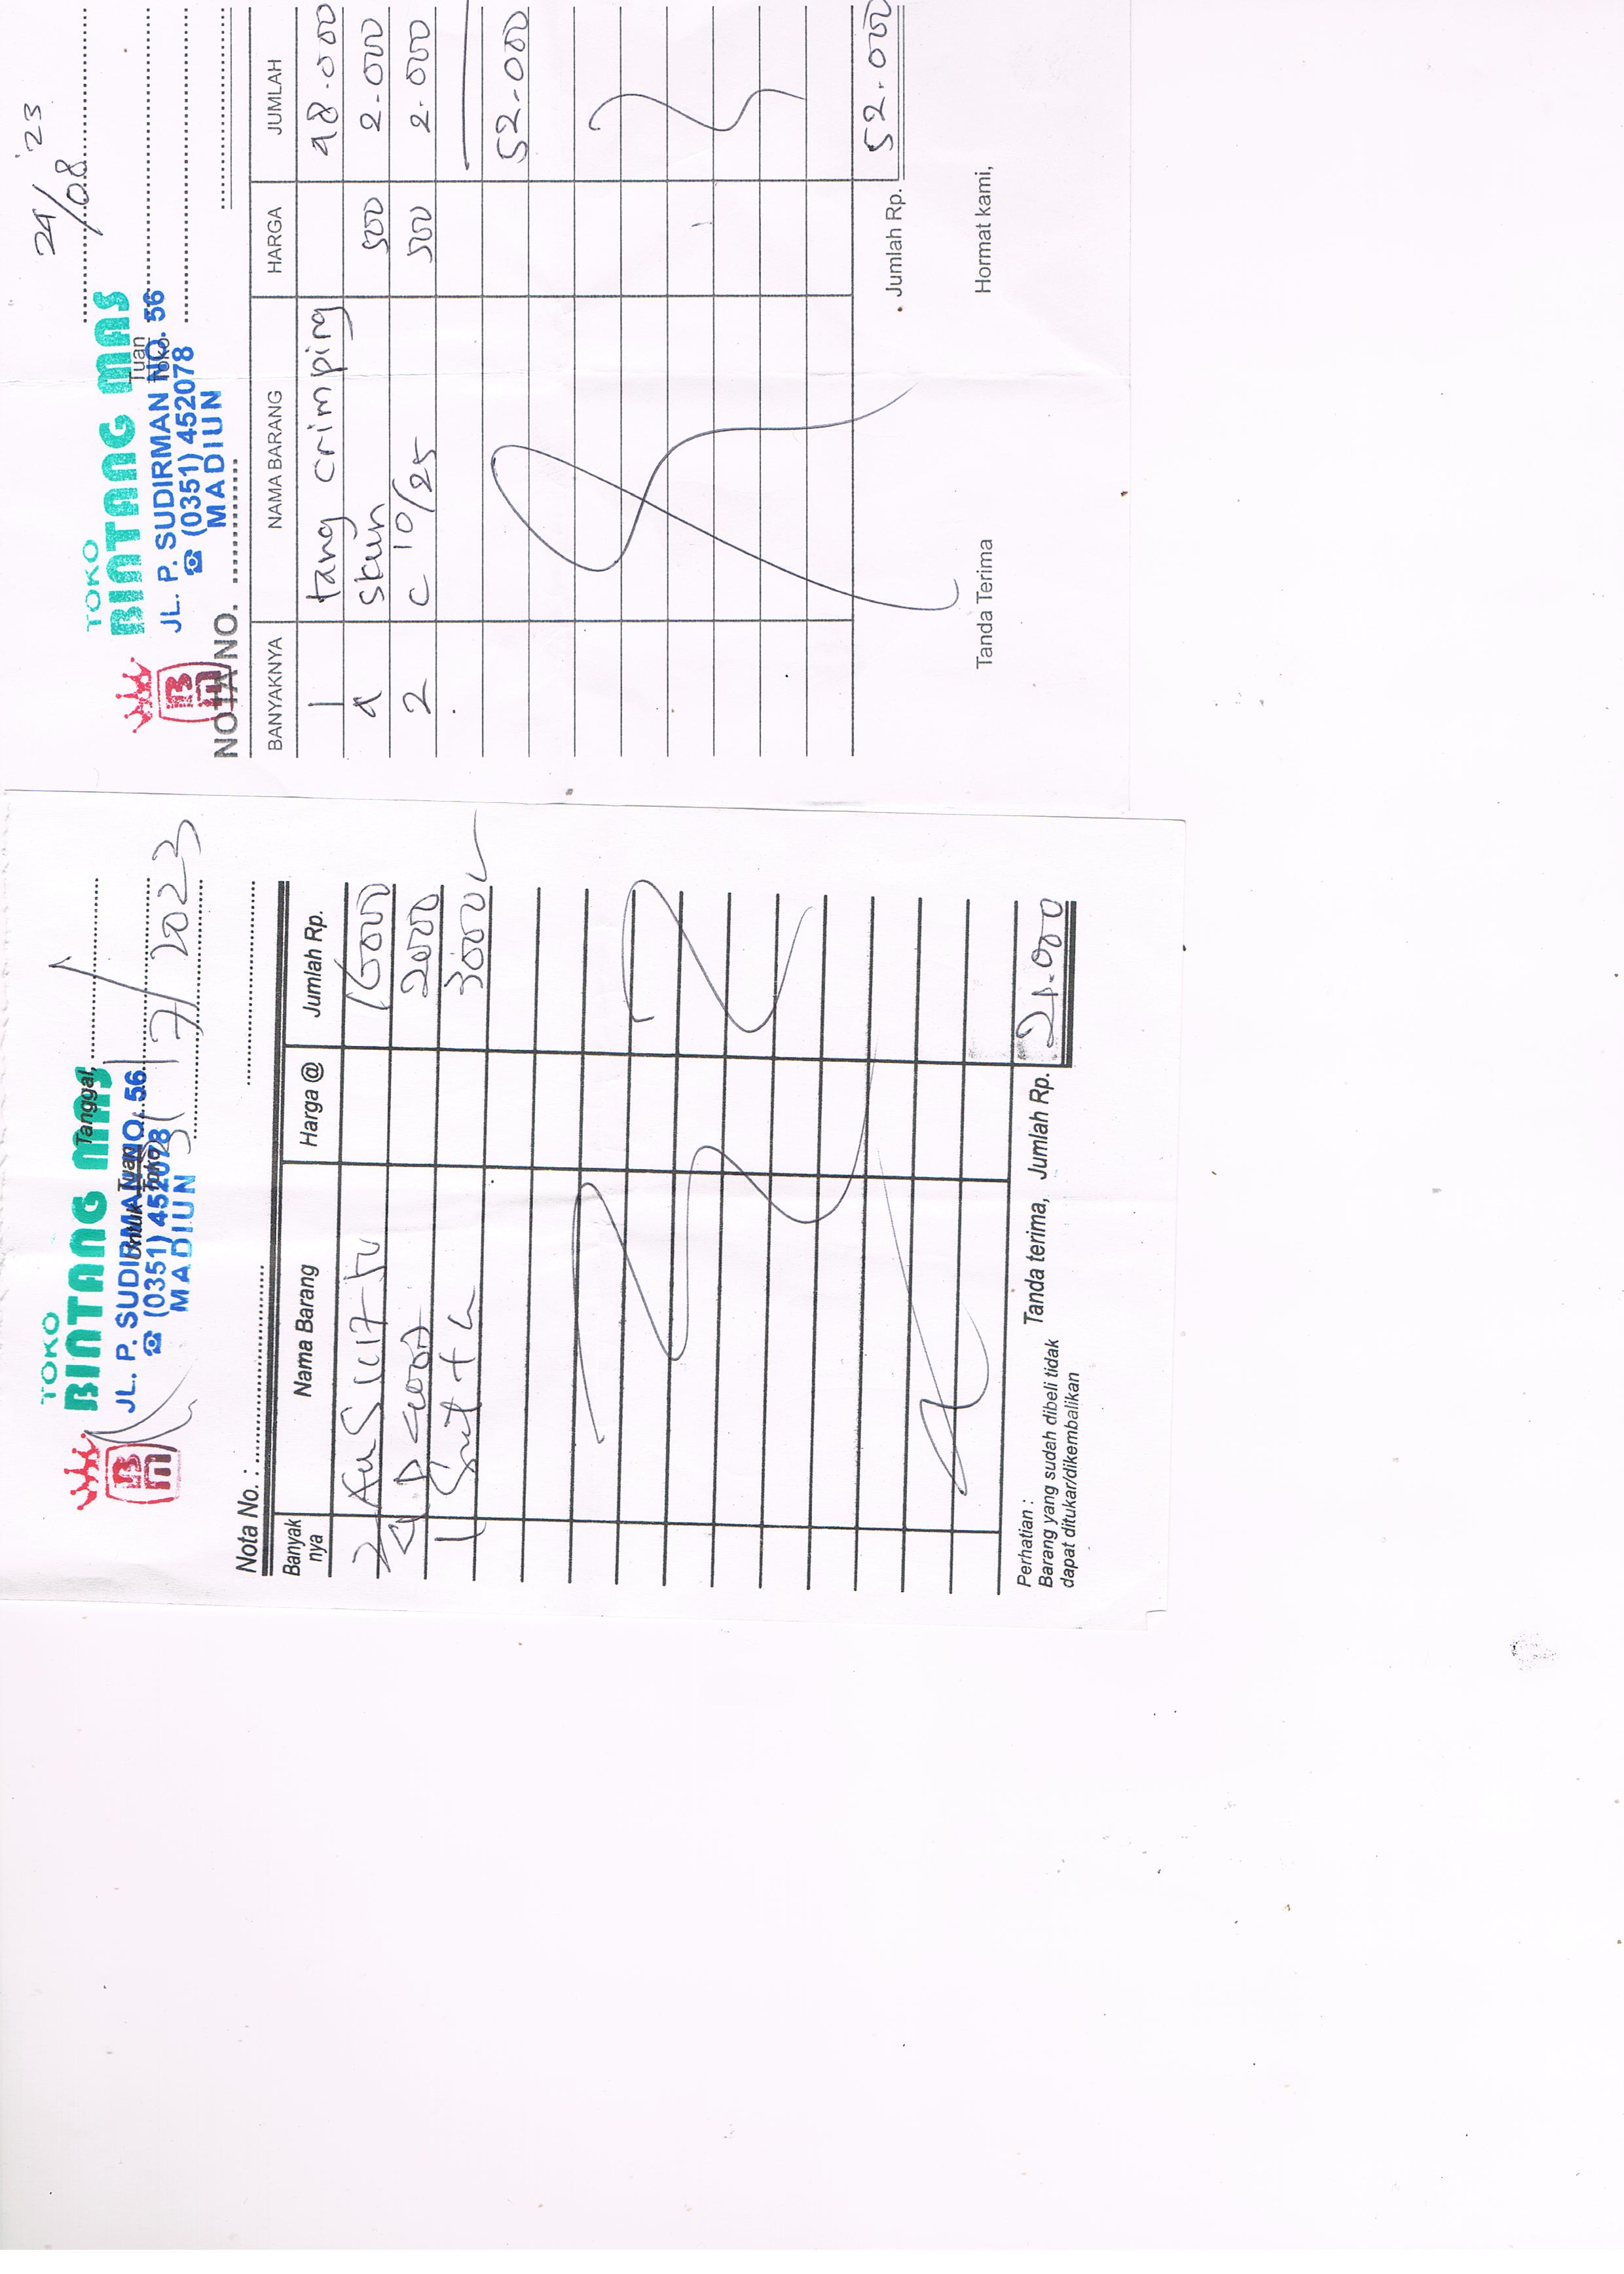
\includegraphics[width=0.8\textwidth]{images/komponen1}
	\end{figure}

	\begin{figure}[H]
		\centering
		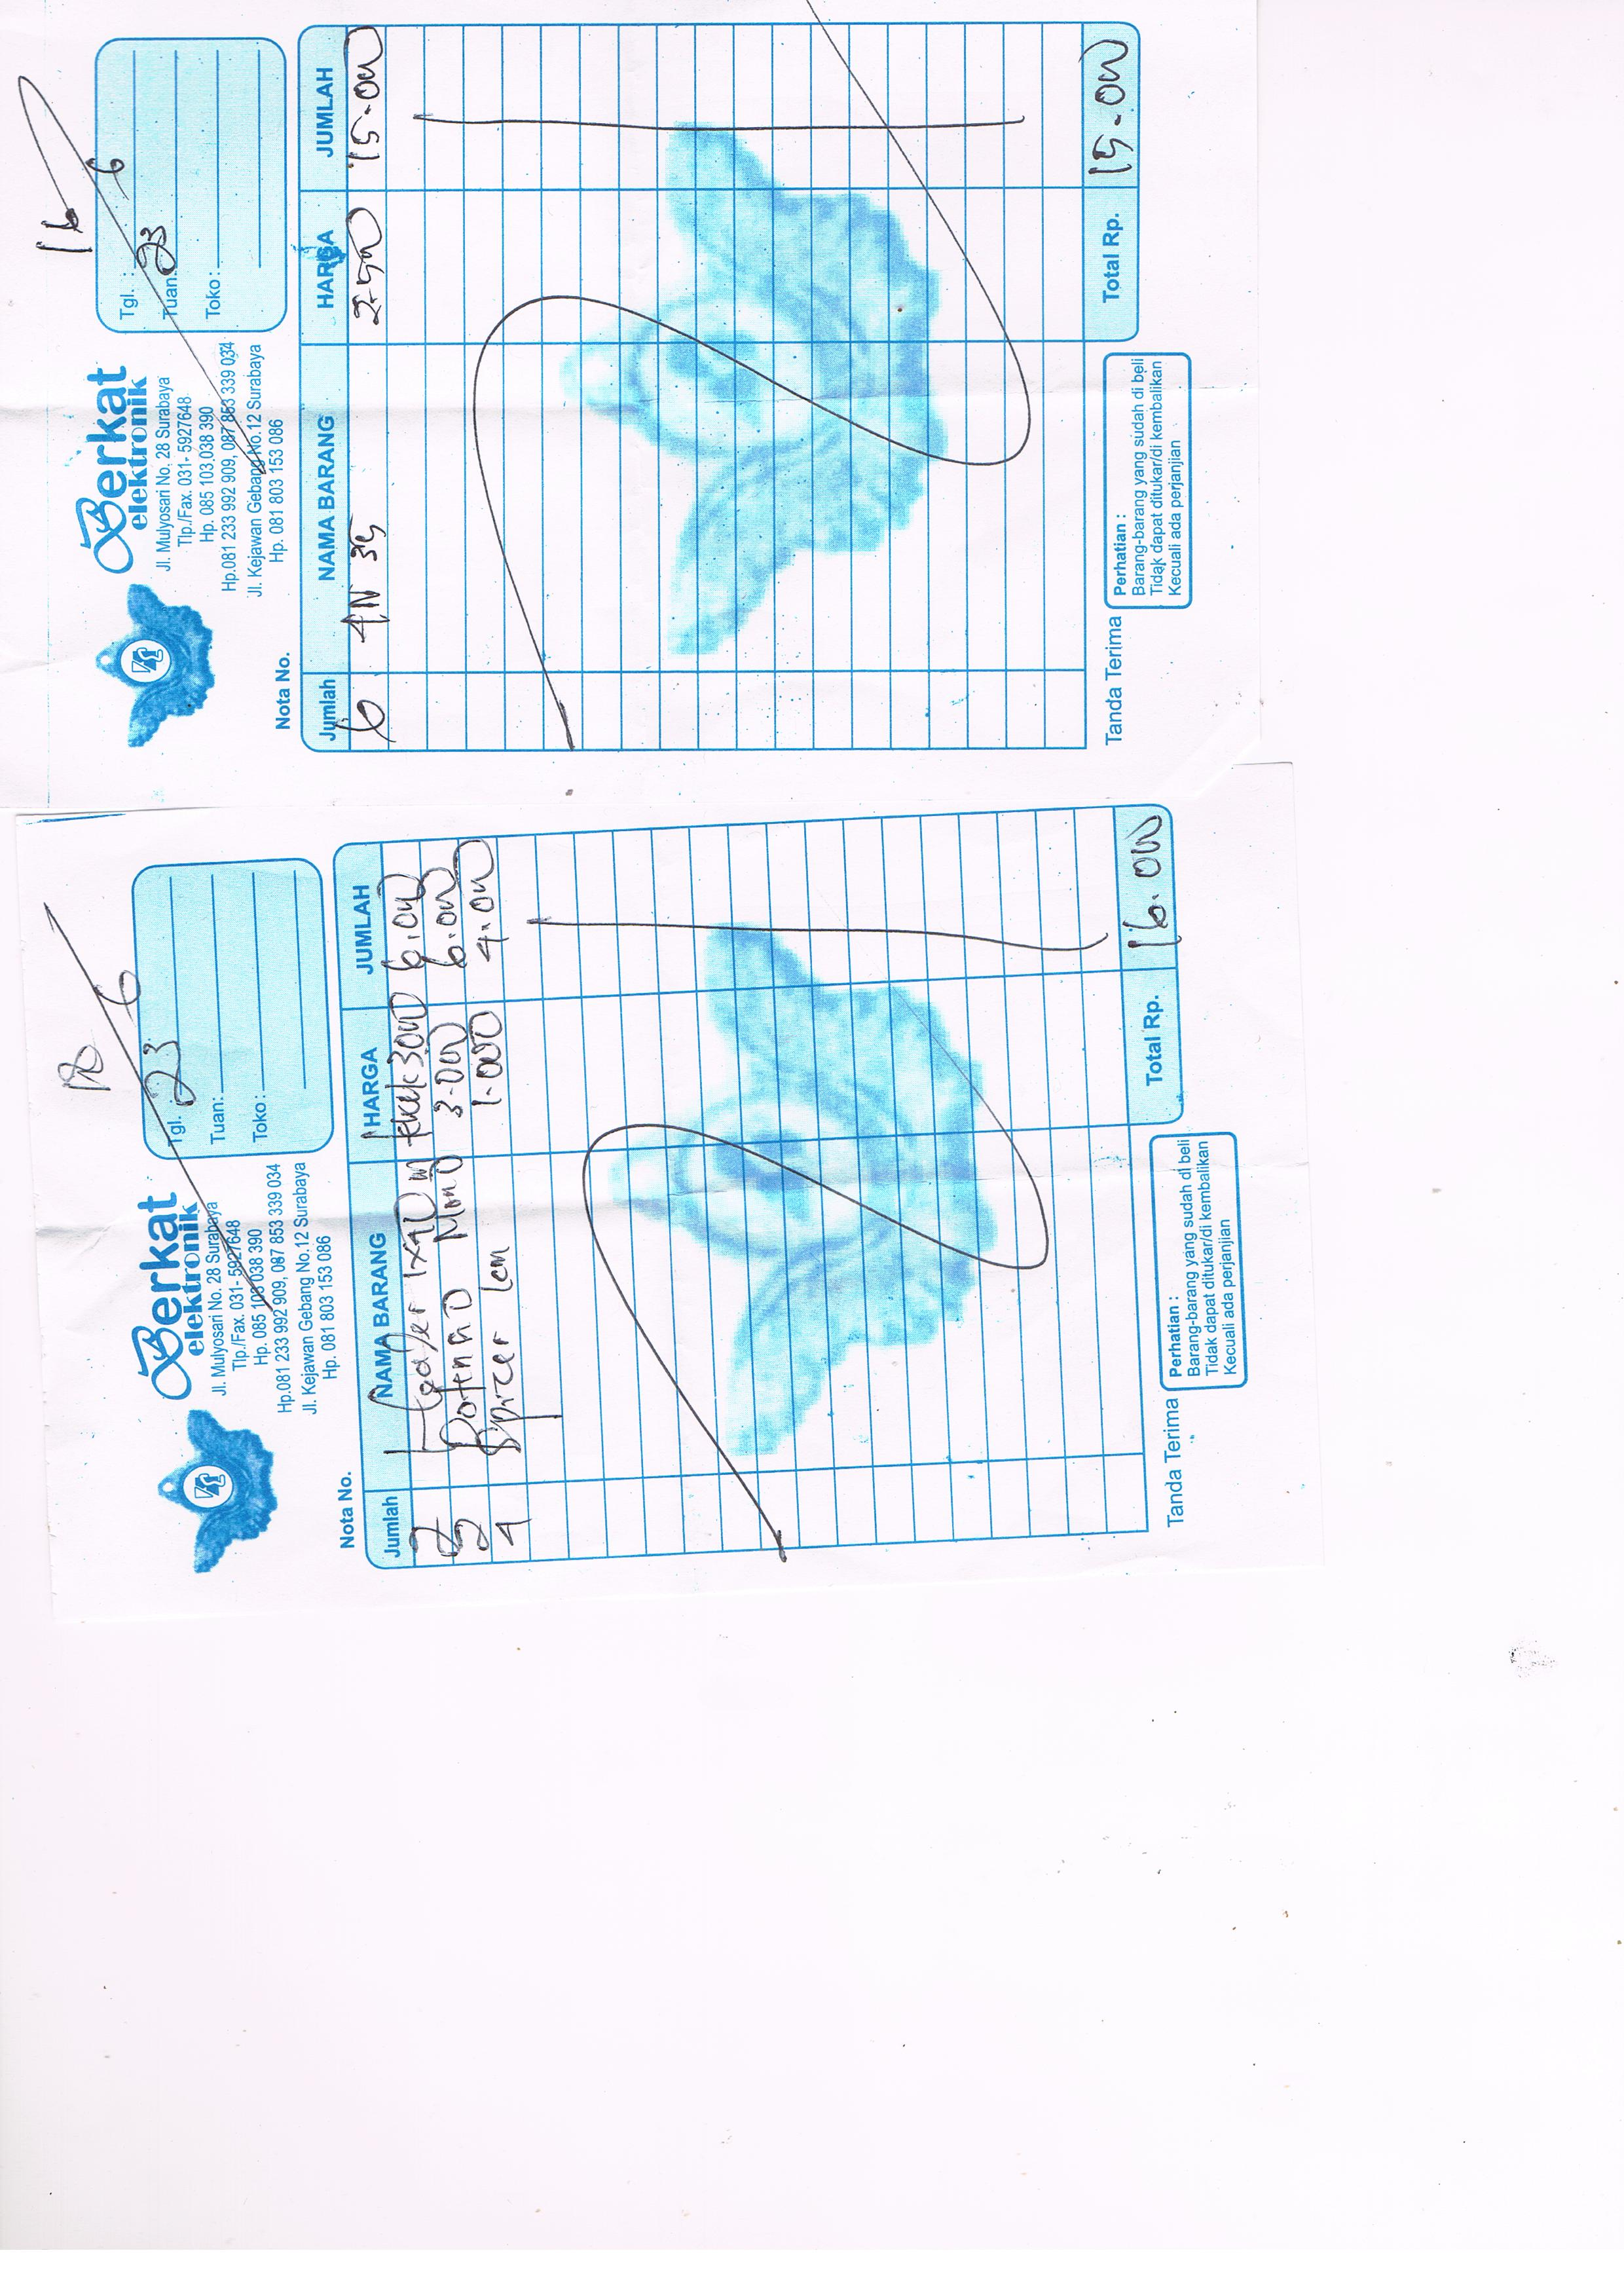
\includegraphics[width=0.8\textwidth]{images/komponen2}
	\end{figure}

	\begin{figure}[H]
		\centering
		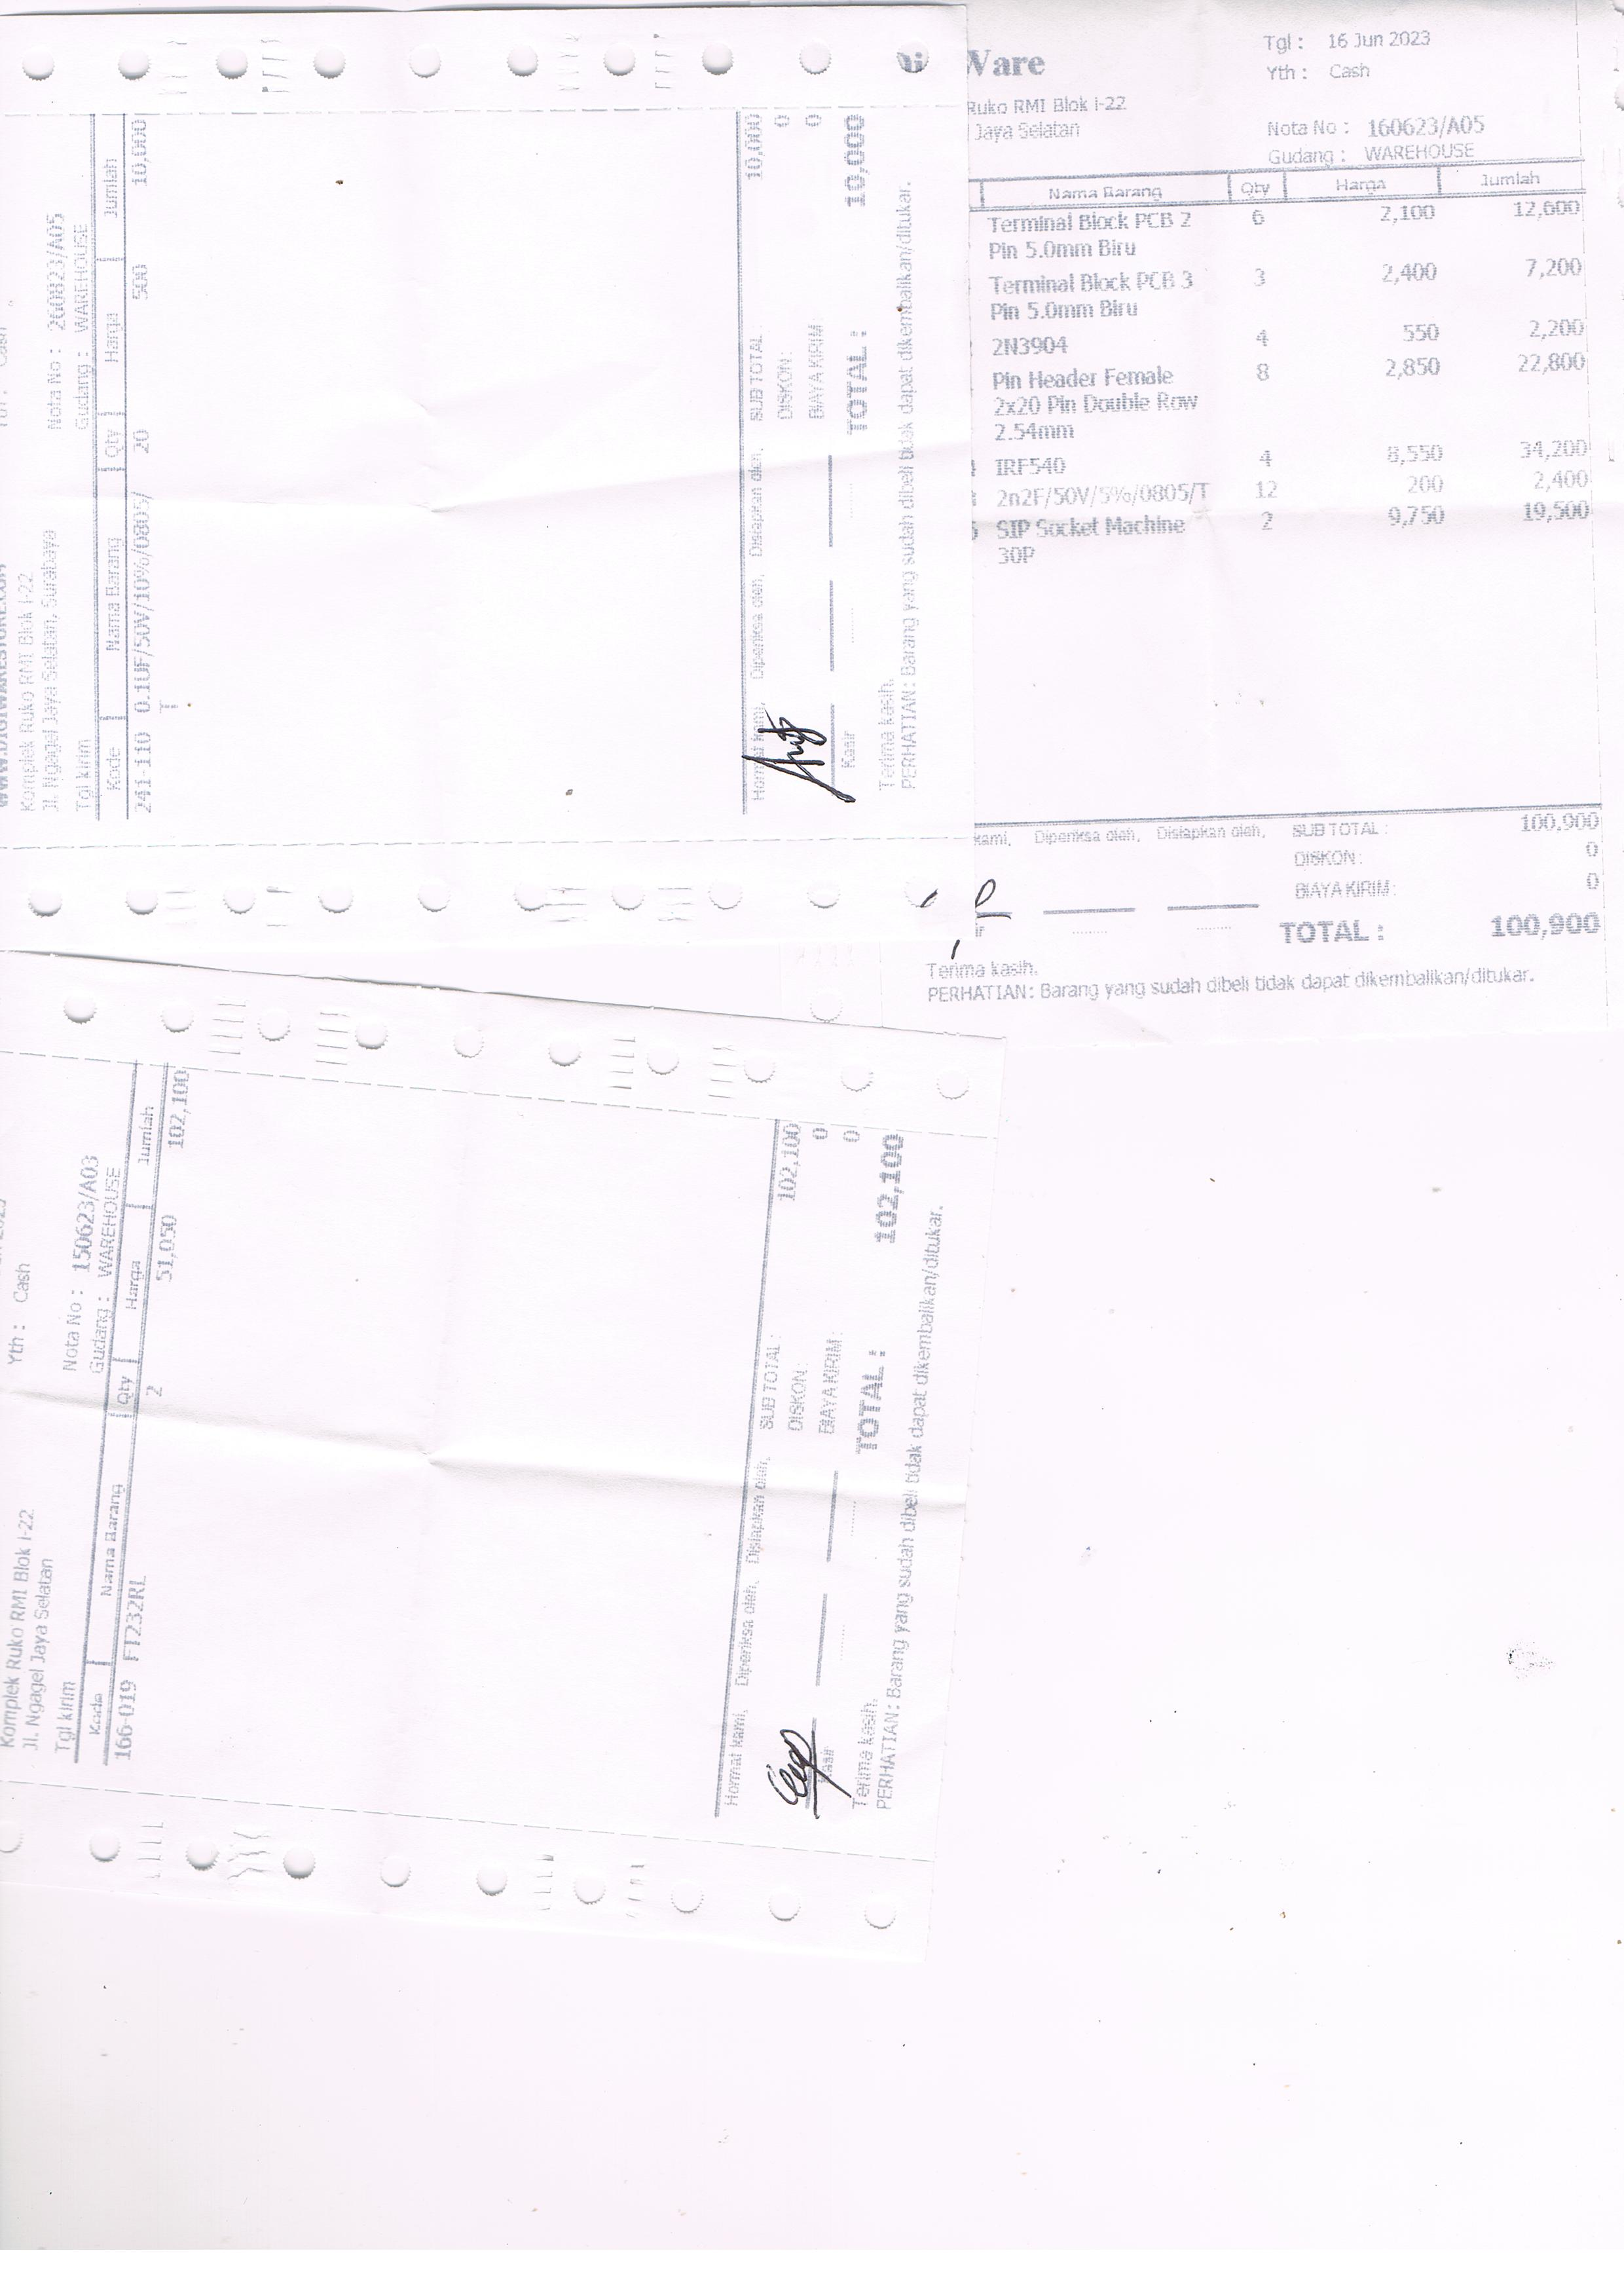
\includegraphics[width=0.8\textwidth]{images/komponen3}
	\end{figure}

	\begin{figure}[H]
		\centering
		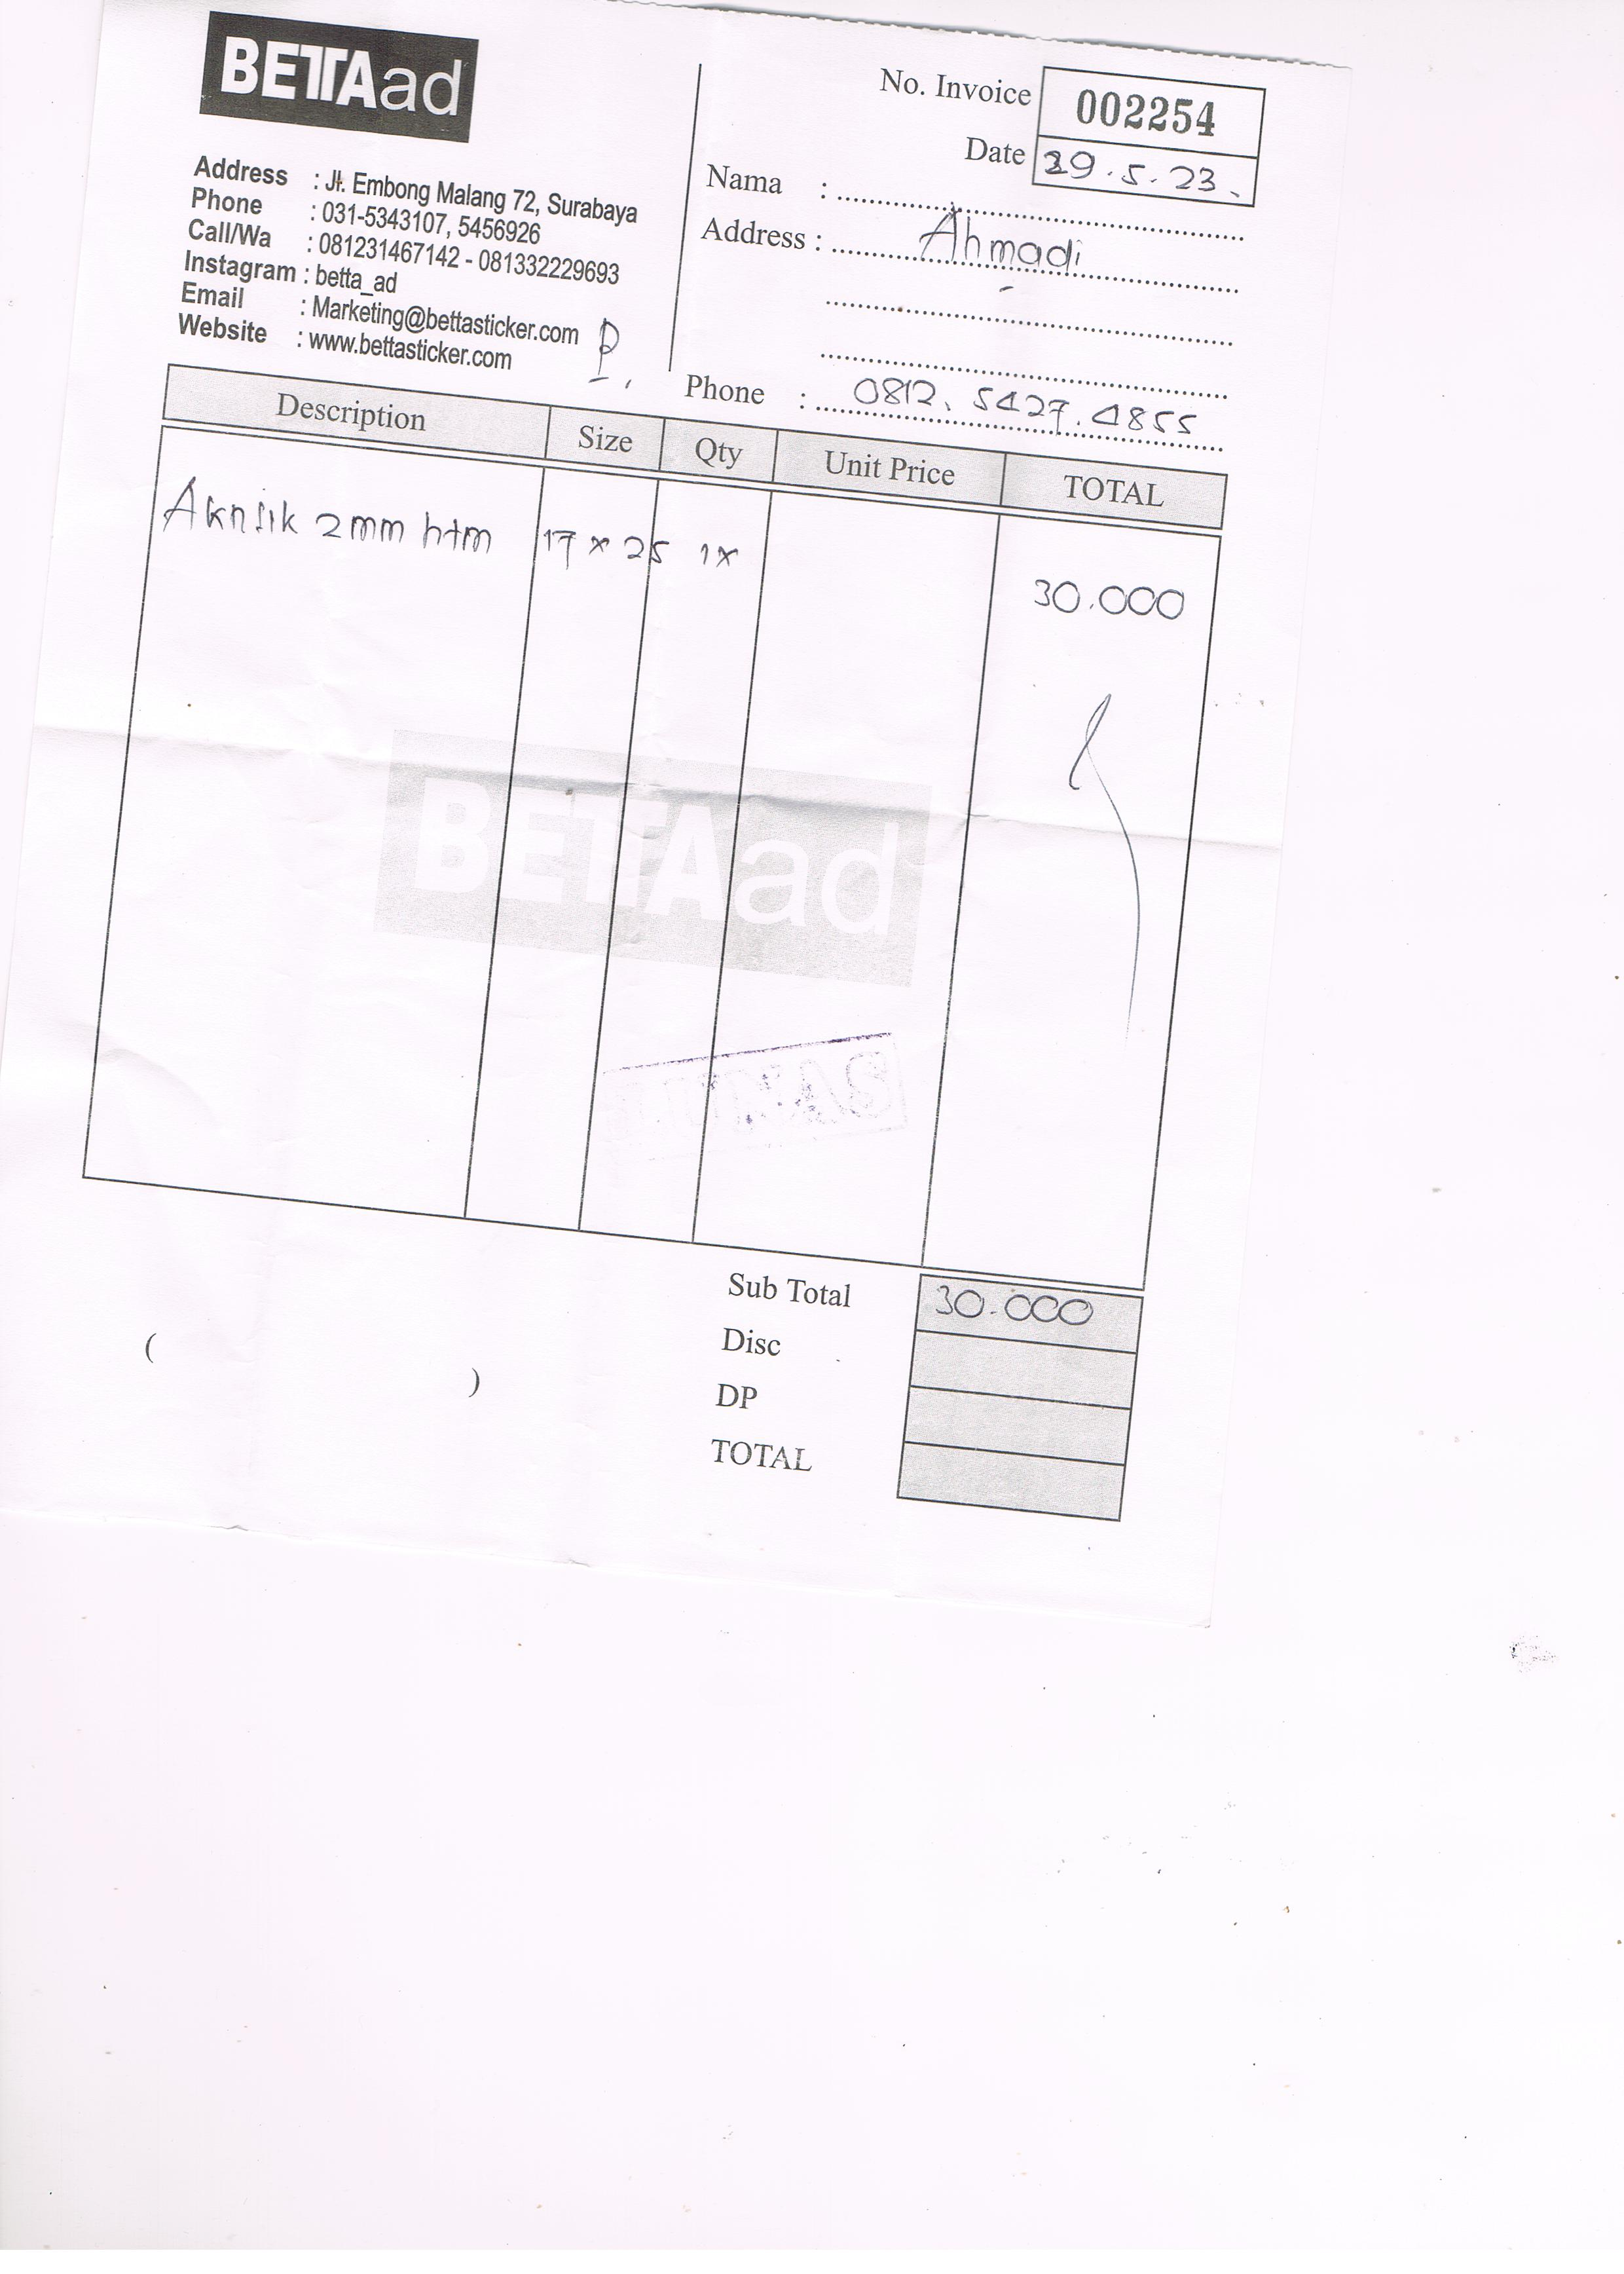
\includegraphics[width=0.8\textwidth]{images/akrilik}
	\end{figure}

	\begin{figure}[H]
		\centering
		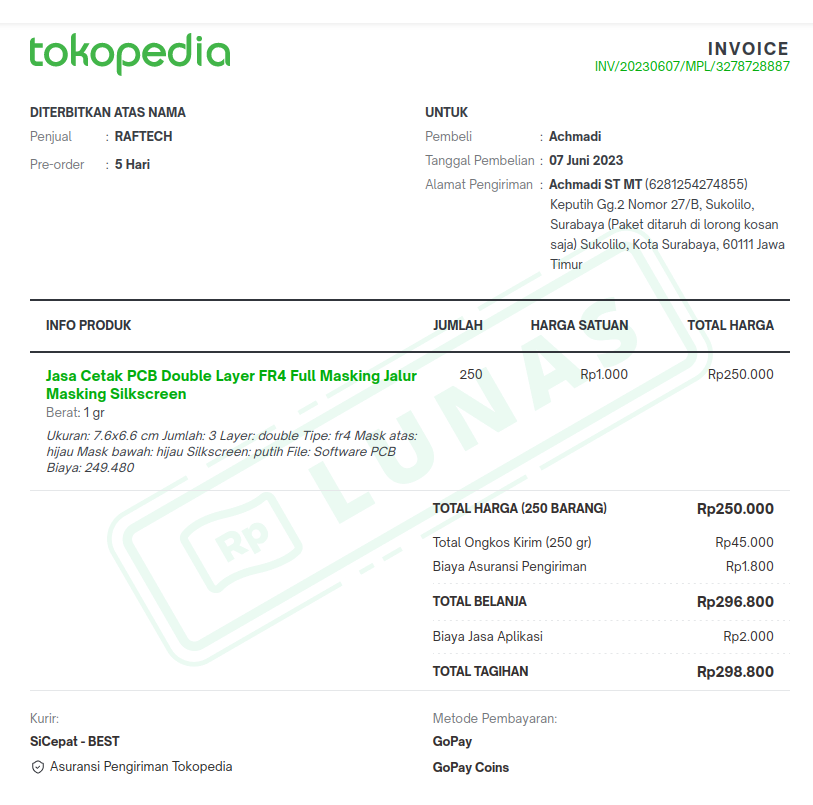
\includegraphics[width=0.8\textwidth]{images/pcb1}
	\end{figure}

	\begin{figure}[H]
		\centering
		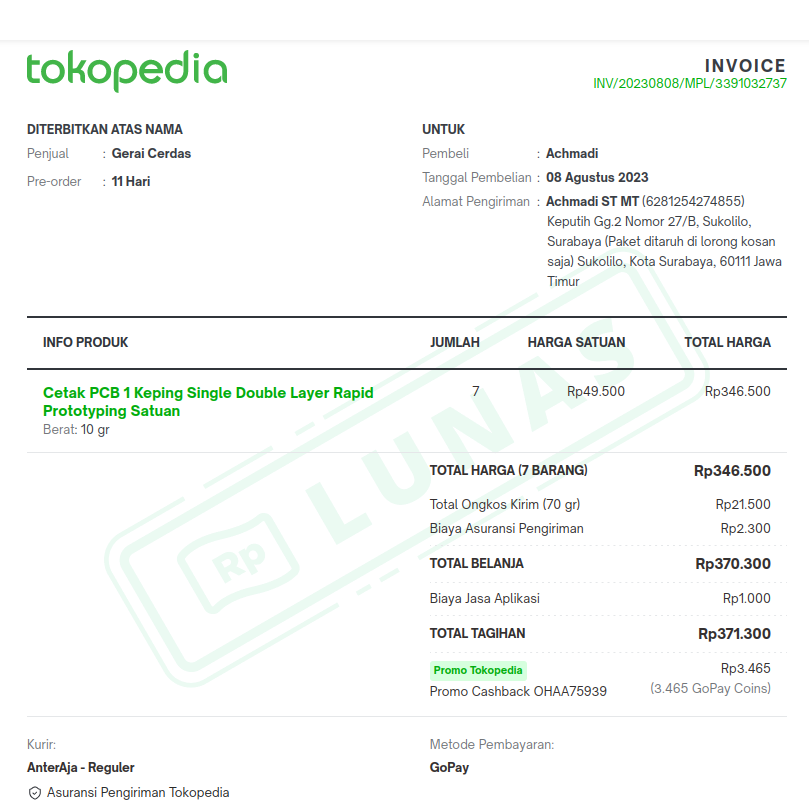
\includegraphics[width=0.8\textwidth]{images/pcb0}
	\end{figure}
	
	\begin{figure}[H]
		\centering
		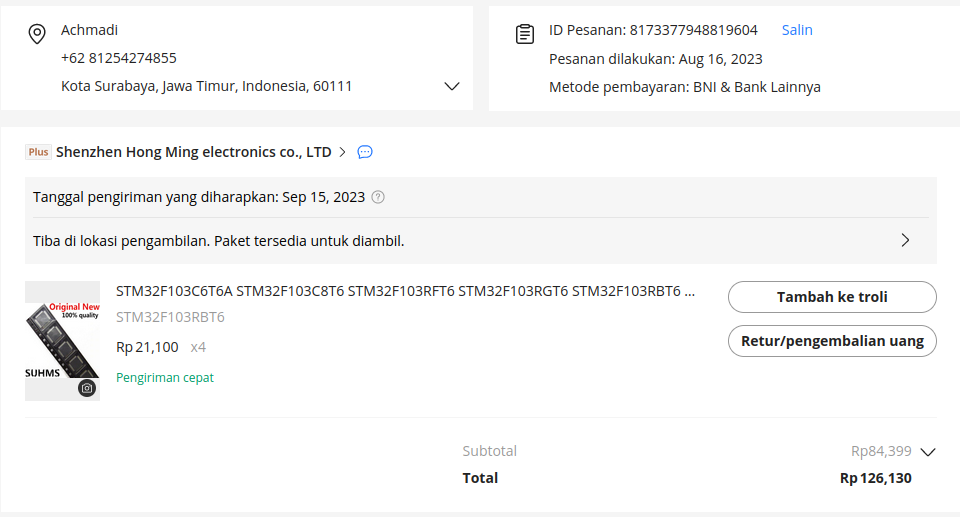
\includegraphics[width=0.8\textwidth]{images/stm32}
	\end{figure}

	\begin{figure}[H]
		\centering
		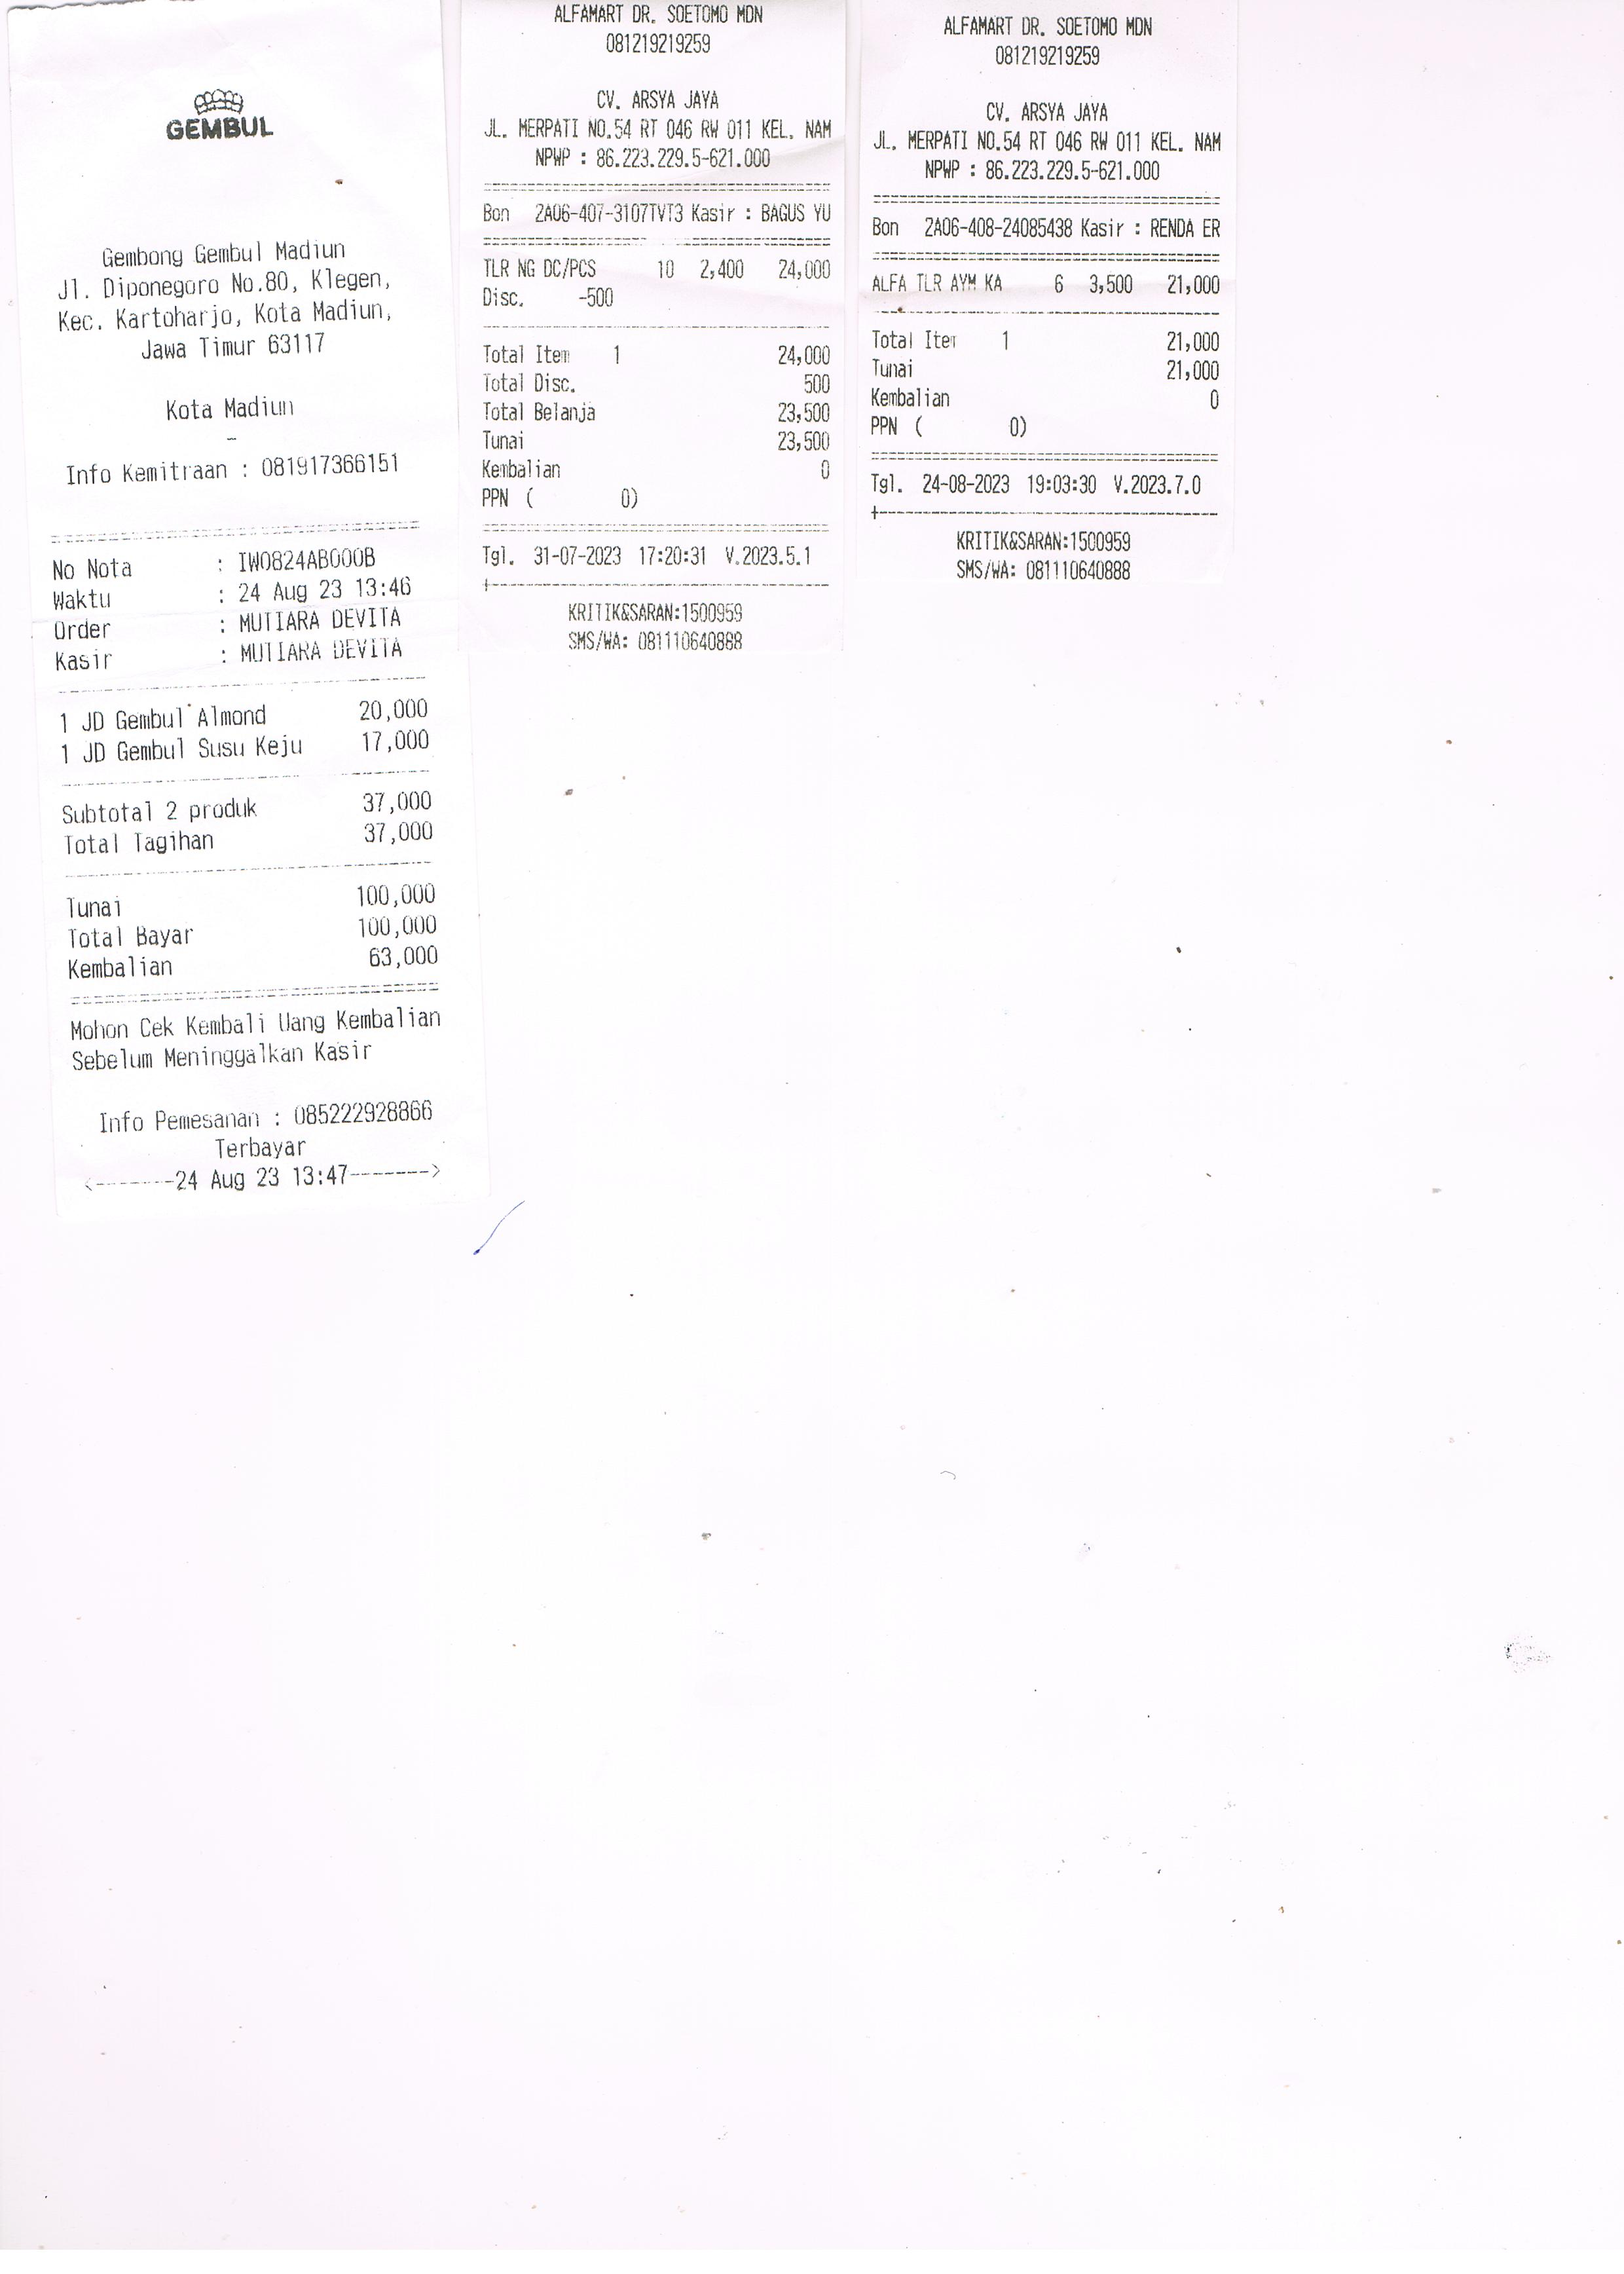
\includegraphics[width=0.8\textwidth]{images/konsum}
	\end{figure}

\end{document}
